\documentclass[12pt]{article}
\usepackage[margin=2.5cm]{geometry}
\usepackage{enumerate}
\usepackage{amsfonts}
\usepackage{amsmath}
\usepackage{fancyhdr}
\usepackage{amsmath}
\usepackage{amssymb}
\usepackage{amsthm}
\usepackage{mdframed}
\usepackage{graphicx}
\usepackage{subcaption}
\usepackage{adjustbox}
\usepackage{listings}
\usepackage{xcolor}
\usepackage{courier}
\usepackage[utf]{kotex}
\usepackage{hyperref}

\definecolor{codegreen}{rgb}{0,0.6,0}
\definecolor{codegray}{rgb}{0.5,0.5,0.5}
\definecolor{codepurple}{rgb}{0.58,0,0.82}
\definecolor{backcolour}{rgb}{0.95,0.95,0.92}

\lstdefinestyle{mystyle}{
    backgroundcolor=\color{backcolour},
    commentstyle=\color{codegreen},
    keywordstyle=\color{magenta},
    numberstyle=\tiny\color{codegray},
    stringstyle=\color{codepurple},
    basicstyle=\ttfamily\footnotesize,
    breakatwhitespace=false,
    breaklines=true,
    captionpos=b,
    keepspaces=true,
    numbers=left,
    numbersep=5pt,
    showspaces=false,
    showstringspaces=false,
    showtabs=false,
    tabsize=1
}

\lstset{style=mystyle}

\pagestyle{fancy}
\renewcommand{\headrulewidth}{0.4pt}
\lhead{CSC 369}
\rhead{Worksheet 2 Solution}

\begin{document}
\title{CSC 369 Worksheet 2 Solution}

\maketitle

\bigskip

\section{Homework (Simulation)}

\begin{enumerate}[1.]
    \item

    \bigskip

    I need to create process trees at each step when the command
    \texttt{./fork.py -s 10} is run.

    \bigskip

    \begin{center}
    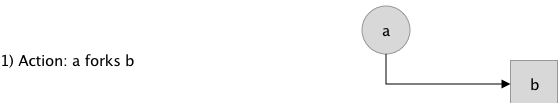
\includegraphics[width=\linewidth]{images/worksheet_2_solution_1.png}
    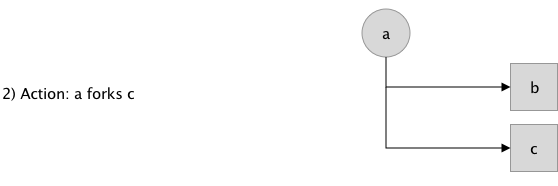
\includegraphics[width=\linewidth]{images/worksheet_2_solution_2.png}
    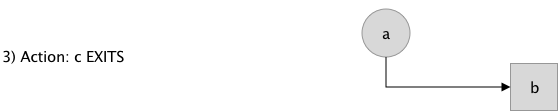
\includegraphics[width=\linewidth]{images/worksheet_2_solution_3.png}
    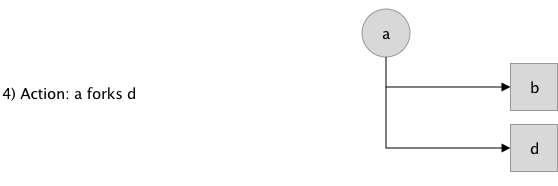
\includegraphics[width=\linewidth]{images/worksheet_2_solution_4.png}
    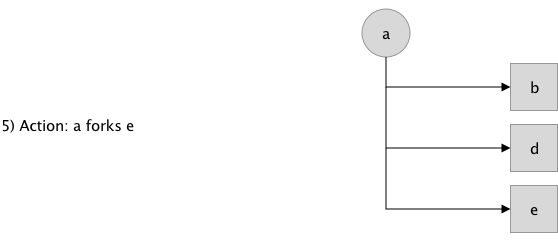
\includegraphics[width=\linewidth]{images/worksheet_2_solution_5.png}
    \end{center}

    \underline{\textbf{Notes}}

    \begin{itemize}
        \item \textbf{fork()}
        \begin{itemize}
            \item Is used to create a new process
            \item \textbf{Creator} $\to$ parent process
            \item \textbf{Newly Created} $\to$ child process
            \item Child process is nearly identical to parent process
        \end{itemize}

        \item \textbf{exec()}

        \begin{itemize}
            \item Allows a child to break free from its similarity to its parent and execute an entirely new program.
        \end{itemize}


        \item \textbf{wait()}
        \begin{itemize}
            \item Is used to let parent code delay its execution until the child finishes
            executing.
            \item Makes the output deterministic
        \end{itemize}
    \end{itemize}

    \item

    \bigskip

    I need to write what the resulting final process trees will look like as the
    fork-percentage changes. Here I ran command (\texttt{./fork.py -s 10 -a 10 -f 0.1} and \texttt{./fork.py -s 10 -a 10 -f 0.9})

    \underline{\textbf{Notes}}

    \begin{itemize}
        \item \texttt{./fork.py -s 10 -a 10 -f 0.1}

        \begin{center}
        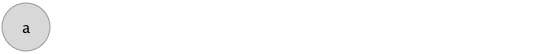
\includegraphics[width=\linewidth]{images/worksheet_2_solution_6.png}
        \end{center}

        \item \texttt{./fork.py -s 10 -a 10 -f 0.9}

        \begin{center}
        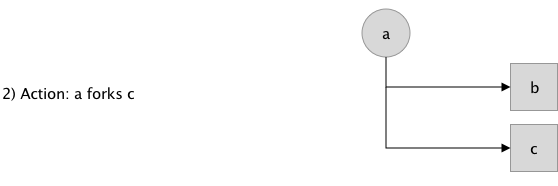
\includegraphics[width=\linewidth]{images/worksheet_2_solution_7.png}
        \end{center}

        \begin{center}
        \end{center}
    \end{itemize}

    Based on the diagram above, I can deduce that the lower the fork percentage,
    the more likely that \texttt{exit()} is executed by the childmost process, and the
    final tree will either have a single node or none.

    \bigskip

    On the other hand, the higher the fork-percentage is, the more likely that \texttt{fork()}
    is executed by the childmost process, and the final tree will have nodes that are deeply nested.
\end{enumerate}

\newpage

\section{Homework (Code)}

\begin{enumerate}[1.]
    \item
\end{enumerate}

\end{document}